\message{ !name(diag_nlr-grammar-2cell.tex)}\documentclass[tikz, preview]{standalone}
\usepackage{amsfonts, amsthm, amssymb, amsmath, stmaryrd, etoolbox}
\usepackage{tikz}
\usetikzlibrary{matrix,arrows}
\tikzset{->-/.style={decoration={markings, mark=at position .5 with {\arrow{>}}},postaction={decorate}}}
\tikzset{->-pos/.style={decoration={markings, mark=at position #1 with {\arrow{>}}},postaction={decorate}}}
\tikzset{->-/.style={decoration={markings,mark=at position .5 with {\arrow{>}}},postaction={decorate}}}
\tikzset{->-pos/.style={decoration={markings,mark=at position #1 with {\arrow{>}}},postaction={decorate}}}

\begin{document}

\message{ !name(diag_nlr-grammar-2cell.tex) !offset(1) }
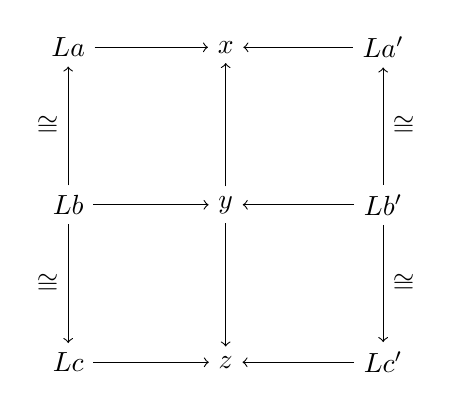
\begin{tikzpicture}
    \node (a) at (-1,1) {$ L a $};
    \node (x) at (1,1) {$ x $};
    \node (a') at (3,1) {$ L a'$};
    \node (b) at (-1,-1) {$ L b $};
    \node (y) at (1,-1) {$ y $};
    \node (b') at (3,-1) {$ Lb' $};
    \node (c) at (-1,-3) {$ L c $};
    \node (z) at (1,-3) {$ z $};
    \node (c') at (3,-3) {$ L c' $};
% 
    \draw [->] (a) to (x);
    \draw [->] (a') to (x);
    \draw [->] (b) to (y);
    \draw [->] (b') to (y);
    \draw [->] (c) to (z);
    \draw [->] (c') to (z);
    \draw [->] (b) to node [left] {$ \cong $} (a);
    \draw [->] (b) to node [left] {$ \cong $} (c);
    \draw [->] (y) to (x);
    \draw [->] (y) to (z);
    \draw [->] (b') to node [right] {$ \cong $} (a');
    \draw [->] (b') to node [right] {$ \cong $} (c');
  \end{tikzpicture}
\message{ !name(diag_nlr-grammar-2cell.tex) !offset(2) }

\end{document}
